% !TEX root =  ../00_thesis.tex

% ------------------------------------------------------------------------------
% Global Positioning
The design of a system is not truly completed until the system's performance has been evaluated. This evaluation must be performed in a way that can be reproduced by others to build confidence in the performance claims.
In this dissertation, we study the design of wireless \CPS and we therefore are directly concerned by the challenge of performing reproducible performance evaluation of networking protocols.
Thus, in this chapter, we tackle the challenge of reproducibility in experimental networking research in general, beyond the sole context of low-power wireless networking (the main focus of this dissertation).
% The \triscale framework presented here is applicable to networking in general~(\cref{fig:chapter_triscale}); as such, the scope of this chapter extends


% ------------------------------------------------------------------------------
% Context
Achieving reproducibility in networking experiments requires a concrete methodology, which is currently missing.
The design and data analysis of experiments raise questions such as: How many runs to perform? How to account for the variability of networking experiments?
Despite the best intentions, researchers often answer these questions differently, which impairs the reproducibility of the entire evaluation.
Moreover, it is currently unclear how to formalize reproducibility, let alone assess whether performance evaluation results are ``reproducible'' or not.

% ------------------------------------------------------------------------------
% What is the problem?

\begin{figure}
  \centering
  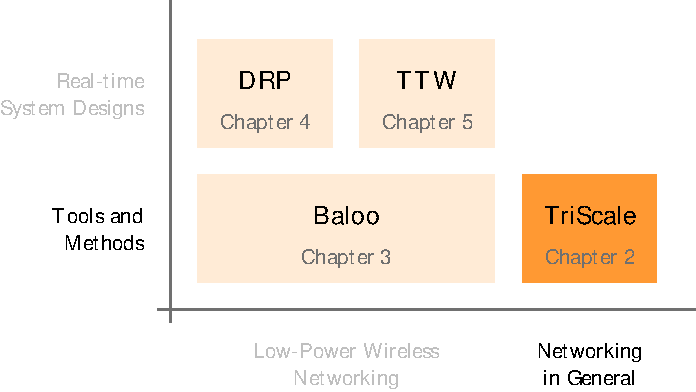
\includegraphics[scale=0.9]{chapter_triscale}
  \caption{This chapter presents \triscale, a framework supporting reproducible evaluations in networking research in general, beyond the sole context of low-power wireless.}
  \label{fig:chapter_triscale}
\end{figure}

% ------------------------------------------------------------------------------
% Claim
\fakepar{Claim}
We contribute to make experimental networking research more rigorous and more reproducible.
For the first time, we go beyond simple guidelines and propose a concrete methodology for designing networking experiments and analyzing their data.
We leverage this methodology to propose the first formalized definition of reproducibility for networking experiments.
Finally, we implement our methodology in a framework called \triscale, a first-of-its-kind tool that assists researchers by streamlining the design process and automating the data analysis.

\pagebreak
% ------------------------------------------------------------------------------
% Corresponding reference(s)
\begin{publi}

  The material from this chapter builds upon the work from Antonios Koskinas~\cite{koskinas2019reproducibility}. It relates to the following publications.

  \inlineRef%
  {Towards a Methodology for Experimental Evaluation in Low-Power Wireless Networking}%
  {Romain Jacob, Carlo Alberto Boano, Usman Raza, Marco Zimmerling, Lothar Thiele}%
  {CPS-IoTBench 2019. Montréal, Canada (April 2019)}

  \inlineRef%
  {TriScale: A Framework Supporting Reproducible Performance Evaluations in Networking}%
  {Romain Jacob, Marco Zimmerling, Carlo Alberto Boano,\\
  Laurent Vanbever, Lothar Thiele}%
  {\emph{Under submission.} (2020)}

\end{publi}
